% LaTeX/AMS-LaTeX

\documentclass[a4paper,11pt]{book}

%%% remove comment delimiter ('%') and specify encoding parameter if required,
%%% see TeX documentation for additional info (cp1252-Western,cp1251-Cyrillic)
%\usepackage[cp1252]{inputenc}

%%% remove comment delimiter ('%') and select language if required
%\usepackage[english,spanish]{babel}

\usepackage{amssymb}
\usepackage{amsmath}
\usepackage[dvips]{graphicx}
%%% remove comment delimiter ('%') and specify parameters if required
%\usepackage[dvips]{graphics}

\begin{document}

%%% remove comment delimiter ('%') and select language if required
%\selectlanguage{spanish} 

\noindent 

\noindent 

\noindent 

\noindent 

\noindent  

\noindent  

\noindent 

\noindent 

\noindent 

\noindent 

\noindent 

\noindent 

\noindent 

\noindent 

\noindent 

\noindent 

\noindent 

\noindent 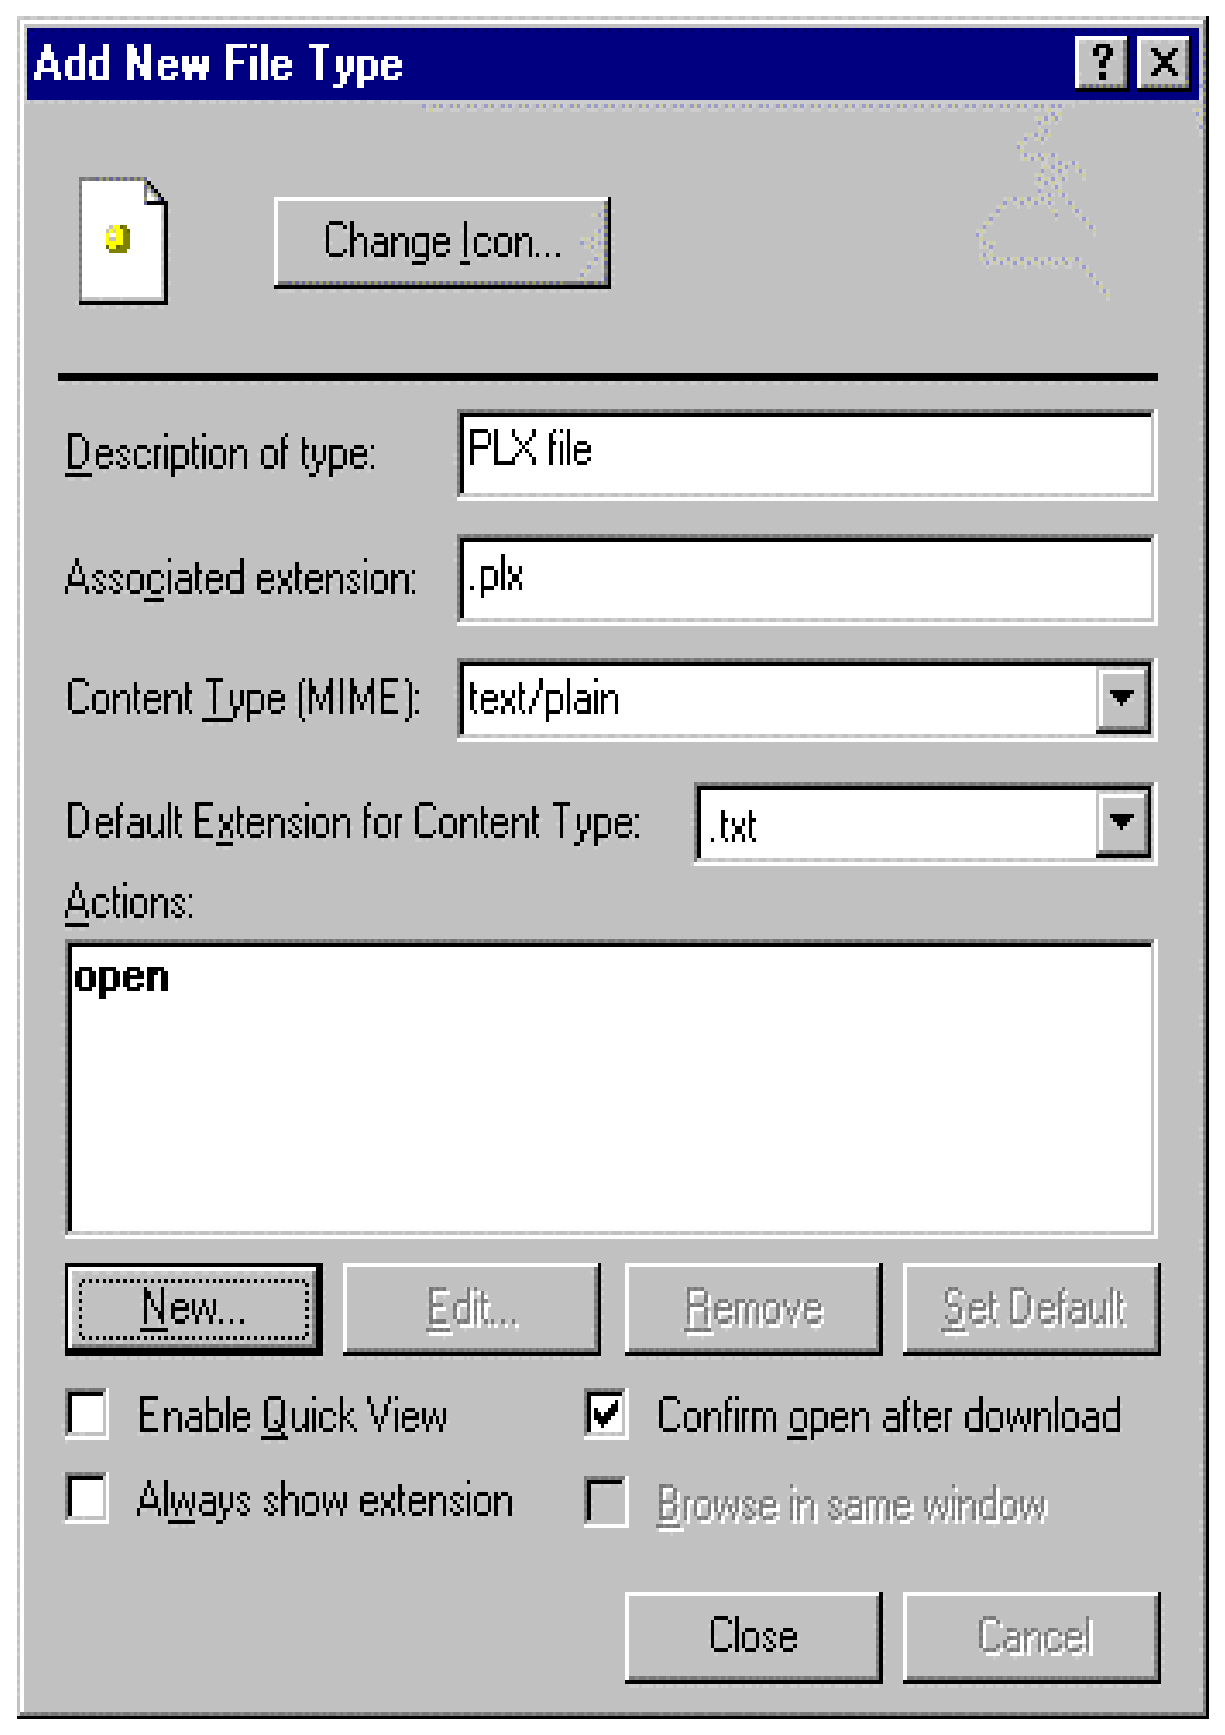
\includegraphics[bb=0mm 0mm 208mm 296mm, width=22.2mm, height=23.1mm, viewport=3mm 4mm 205mm 292mm]{image2.ps}Special Variables

\noindent 

\noindent 

\noindent 

\noindent 

\noindent 

\noindent 

\noindent Default Variables and Parameters

\noindent 

\noindent \textbf{Variable Description}

\noindent 

\noindent \$\_ This  global scalar acts  as a  default  variable  for  function  arguments  and  pattern- searching  space -- with  many common  functions,  if  an  argument  is  left unspecified,  \$\_ will be automatically  assigned,  so,  for  example,  the following statements are equivalent:

\noindent 

\noindent chop(\$\_) and chop

\noindent 

\noindent \$\_   =\~{} m/\textit{expr}/ and m/\textit{expr}/

\noindent 

\noindent @\_ The elements of this array are used to store function arguments, which can be accessed (from within a function definition) as \$\_[\textit{num}]. The array is automatically local to each function.

\noindent 

\noindent @ARGV The elements of this array contain the command line arguments intended for use by the script.

\noindent 

\noindent \$ARGV This contains the name of the current file when reading from the null filehandle

\noindent $<$$>$. ( $<$$>$ is a literal, and defaults to standard input, $<$STDIN$>$, if no arguments are supplied from elements in @ARGV).

\noindent \eject 

\noindent Regular Expression Variables (all read-only)

\noindent 

\noindent \textbf{Variable Description}

\noindent 

\noindent \$(\textit{num}) The scalar  \$\textit{n }contains the substring  matched  to  the  \textit{n}'th  grouped  subpattern

\noindent in  the  last pattern match,  and  remains  in  scope  until  the  next  pattern  match

\noindent with subexpressions.  It  ignores  matched  patterns  occurring  in  nested  blocks  that are already exited.  If there are  no  corresponding  groups,  then  the  undefined

\noindent value  is returned.

\noindent 

\noindent \$\& This  scalar contains the string matched by the last successful pattern match. Once again, this won't include any strings matched in nested blocks. For example:

\noindent 'UnicornNovember' =\~{} /Nov/;

\noindent print \$\&;

\noindent will print Nov. For versions of perl since 5.005, this is not an expensive variable to

\noindent use.

\noindent 

\noindent \$' This scalar holds the substring following whatever was matched by the last successful pattern match. For example, if we say:

\noindent 'UnicornNovember' =\~{} /Nov/;

\noindent \$' will return ember.

\noindent 

\noindent \$` This scalar holds the substring preceding whatever was matched by the last successful pattern match. For example, if we say:

\noindent 'UnicornNovember' =\~{} /Nov/;

\noindent \$` will return Unicorn.

\noindent 

\noindent \$+ This scalar holds the last substring matched to a grouped subpattern in the last

\noindent search. It comes in handy if you're not sure which of a set of alternative subpatterns matched. For example, if you successfully match on /(ab)*\textbar  (bc*)/, then \$+ stores either \$1 or \$2, depending on whether it was the first or second grouped subpattern that matched. For example, following:

\noindent 

\noindent 'UnicornNovember' =\~{} /(Nov)\textbar (Dec)/;

\noindent \$+ will return Nov.

\noindent 

\noindent @+ This array lists the back pointer positions (in the referenced string) of the last successful match. The first element @+[0] contains the pointer's starting position following that match -- each subsequent value corresponds to its position just \textit{after }having matched the corresponding grouped subpattern. For example, following:

\noindent 

\noindent 'UnicornNovember' =\~{} /(U)\textbackslash w?(N)/;

\noindent 

\noindent @+ will return (8,1,8), while following:

\noindent 

\noindent 'UnicornNovember' =\~{} /(Uni)\textbackslash w?(Nov)/;

\noindent 

\noindent @+ will return (10,3,10).

\noindent \eject 

\noindent @- This array lists the front pointer positions (in the referenced string) of the last successful match. The first element @-[0] contains the pointer's starting position prior to that match -- each subsequent value corresponds to its position just \textit{before }having matched the corresponding grouped subpattern. For example following:

\noindent 

\noindent 'UnicornNovember' =\~{} /(Uni)\textbackslash w?(Nov)/;

\noindent 

\noindent @- will return (0,0,7), while following:

\noindent 

\noindent 'UnicornNovember' =\~{} /(Uni)(\textbackslash w?)(Nov)/;

\noindent 

\noindent @- will return (0,0,3,7).

\noindent 

\noindent 

\noindent 

\noindent Input/Output Variables

\noindent 

\noindent \textbf{Variable Description}

\noindent 

\noindent \$. This scalar holds the \textbf{current line number }of the last filehandle on which you performed either a read, seek, or  tell. It is reset when the filehandle is closed.

\noindent 

\noindent NB: $<$$>$ never does an explicit close, so line numbers increase across ARGV files -- also, localizing \$. has the effect of also localizing perl's notion of 'the last read filehandle'.

\noindent 

\noindent \$/ This scalar stores the \textbf{input record separator}, which by default is the newline \textbackslash n. If it's set to "", input will be read one paragraph at a time.

\noindent 

\noindent \$\textbackslash  This scalar stores the \textbf{output record separator }for print -- normally this will just output consecutive records without any separation (unless explicitly included). This variable allows you to set it for yourself. For example:

\noindent 

\noindent \$\textbackslash  = "-"; print "one"; print "two";

\noindent will print one-two-.

\noindent 

\noindent \$\textbar  This corresponds to an internal flag used by perl to determine whether buffering should be used on a program's write/read operations to/from files. If the value is TRUE (\$\textbar  is greater than 0), buffering is disabled.

\noindent 

\noindent \$, This is the \textbf{output field separator }for print -- normally this will just output consecutive fields without any separation (unless explicitly included). This variable allows you to set it for yourself. For example:

\noindent \eject 

\noindent \$, = "-";

\noindent print "one","two";

\noindent 

\noindent will print one-two.

\noindent 

\noindent 

\noindent 

\noindent 

\noindent 

\noindent 

\noindent \textit{Table continued on following page}

\noindent \eject 

\noindent 

\noindent \textbf{Variable Description}

\noindent 

\noindent \$" This is the \textbf{output field separator }for array values interpolated into a double- quoted string (or similar interpreted string) -- the default is a space. For example:

\noindent 

\noindent \$" = "-";

\noindent @ar = ("one", "two", "three");

\noindent print "@ar";

\noindent 

\noindent will print one-two-three.

\noindent 

\noindent 

\noindent 

\noindent Filehandle/format Variables

\noindent 

\noindent \textbf{Variable Description}

\noindent 

\noindent \$\# This holds the \textbf{output format }for printed numbers.

\noindent \textbf{NB: The use of this variable has been deprecated.}

\noindent \$\textbar  This corresponds to an internal flag used by perl to determine whether \textbf{buffering }should be used on a program's write/read operations to/from files -- if its value is TRUE (\$\textbar  is greater than 0), then buffering is disabled.

\noindent \$\% The current page number of the selected output channel.

\noindent \$= The current \textbf{page length}, measured in printable lines -- the default is 60.

\noindent This only becomes important when a top-of-page format is invoked -- if a write command doesn't fit into a given number of lines, then the top-of-page format is used, before any printing past the page length continues.

\noindent \$- The number of lines left on a page -- when a page is finished, it's given the value of

\noindent \$=, and is then decremented for each line outputted.

\noindent \$\~{} The currently selected \textbf{format name }-- the default is the name of the filehandle.

\noindent \$\^{} The name of the \textbf{top-of-page format}.

\noindent \$: The set of characters after which a string may be broken to fill continuation fields

\noindent (starting with \^{}) in a format -- default is '   \textbackslash n-' to break on whitespace or hyphens.

\noindent \$\^{}L This holds a character that is used by a format's output to request a form feed --

\noindent default is \textbackslash f.

\noindent 

\noindent 

\noindent 

\noindent Error Variables

\noindent 

\noindent \textbf{Variable Description}

\noindent 

\noindent \$? This holds the status value returned by the last pipe close, backtick (``) command,

\noindent or system() operator.

\noindent 

\noindent \$@ This holds the \textbf{syntax error message }from the last eval() command -- it evaluates

\noindent to null if the last eval() parsed and executed correctly (although the operations you invoked may have failed in the normal fashion).

\noindent \eject 

\noindent \$! If used in a numeric context, this returns the current value of \textit{errno}, with all the usual caveats. (so you shouldn't depend on \$! to have any particular value unless you've

\noindent got a specific error return indicating a system error.)

\noindent 

\noindent If used in a string context, it returns the corresponding system error string. You can assign a set \textit{errno }value to \$! if, for instance, you want it to return the string for that error number, or you want to set the exit value for the die() operator.

\noindent 

\noindent \$\^{}E This returns an \textbf{extended error message}, with information specific to the current operating system. At the moment, this only differs from \$! under VMS, OS/2, and Win32 (and for MacPerl). On all other platforms, \$\^{}E is always the same as \$!.

\noindent 

\noindent 

\noindent 

\noindent System Variables

\noindent 

\noindent \textbf{Variable Description}

\noindent 

\noindent \$\$ The \textbf{process ID }(pid) of the Perl process running the current script.

\noindent 

\noindent \$$<$ The \textbf{real user ID }(uid) of the current process.

\noindent 

\noindent \$$>$ The \textbf{effective uid }of the current process.

\noindent 

\noindent NB: \$$<$ and \$$>$ can only be swapped on machines supporting setreuid().

\noindent 

\noindent \$( The \textbf{real group ID }(gid) of the current process.

\noindent 

\noindent \$) The \textbf{effective group ID }(gid) of the current process.

\noindent 

\noindent \$0 (zero) The name of the file containing the Perl script being executed.

\noindent 

\noindent \$\^{}X The name that the perl binary was executed as.

\noindent 

\noindent \$] The version number of the perl interpreter, including patchlevel / 1000 -- can be

\noindent used to determine whether the interpreter executing a script is within the right range

\noindent of versions.

\noindent 

\noindent See also use VERSION and require VERSION for a way to fail if the interpreter

\noindent is too old.

\noindent 

\noindent \$\^{}O The name of the operating system under which this copy of perl was built, as determined during the configuration process -- identical to \$Config\{'osname'\}.

\noindent 

\noindent \$\^{}T The time at which the current script began running, in seconds since the beginning

\noindent of 1970. Values returned by -M, -A, and -C filetests are based on this value.

\noindent 

\noindent \$\^{}W The current value of the warning switch, either TRUE or FALSE.

\noindent 

\noindent \%ENV Your current environment -- altering its value changes the environment for child processes.

\noindent 

\noindent \%SIG Used to set handlers for various signals.

\noindent \eject 

\noindent Others

\noindent 

\noindent \textbf{Variable Description}

\noindent 

\noindent @INC A list of places to look for Perl scripts for evaluation by the do EXPR, require,

\noindent or use constructs.

\noindent 

\noindent \%INC Contains entries for each filename that has been included via do or require. The key is the specified filename, and the value the location of the file actually found.

\noindent The require command uses this array to determine whether a given file has already been included.

\noindent \eject Special Variables

\noindent \eject 

\noindent 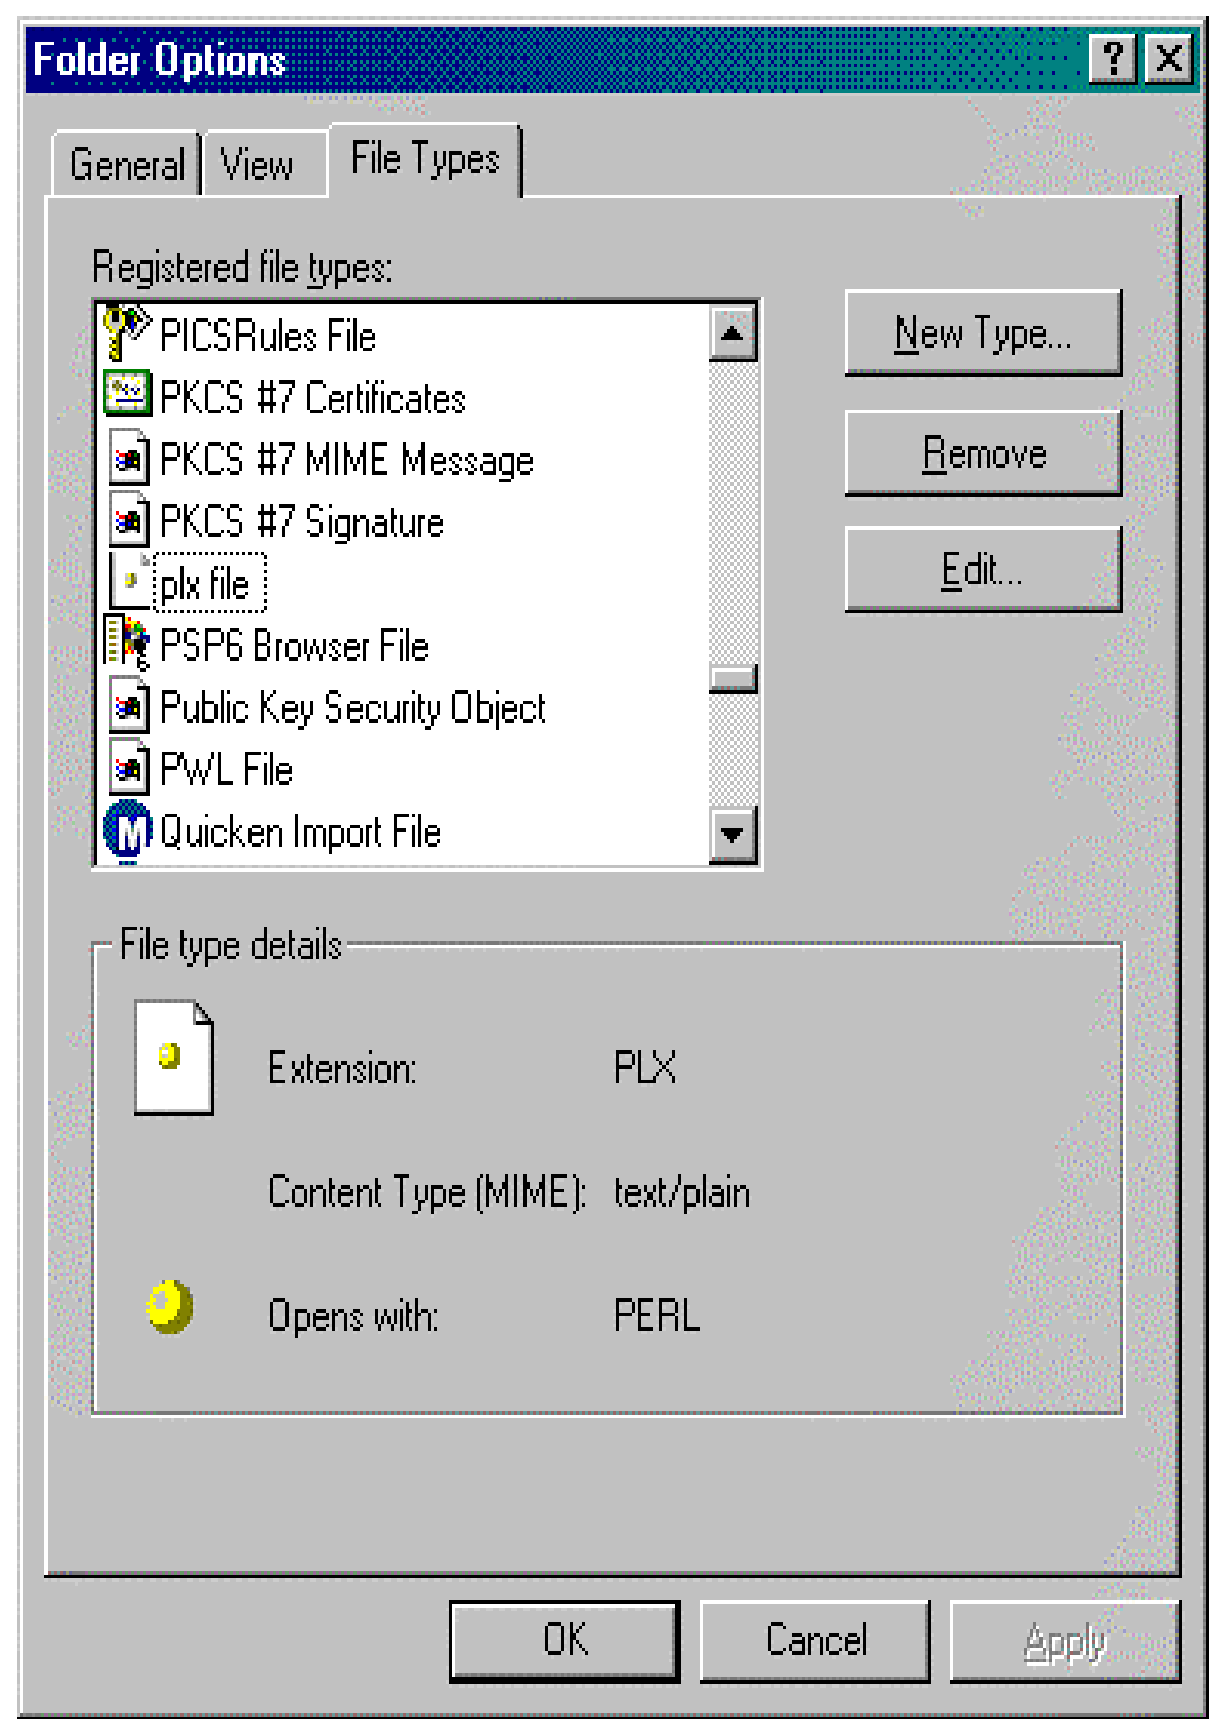
\includegraphics[bb=0mm 0mm 208mm 296mm, width=185.2mm, height=196.3mm, viewport=3mm 4mm 205mm 292mm]{image3.ps}

\noindent 

\noindent This work is licensed under the Creative Commons Attribution-NoDerivs-NonCommercial License. To view a copy of this

\noindent license, visit http://creativecommons.org/licenses/by-nd-nc/1.0 or send a letter to Creative Commons, 559 Nathan Abbott Way, Stanford, California 94305, USA.

\noindent 

\noindent The key terms of this license are:

\noindent 

\noindent Attribution: The licensor permits others to copy, distribute, display, and perform the work. In return, licensees must give the original author credit.

\noindent 

\noindent No  Derivative  Works: The licensor permits others to copy, distribute, display and perform only unaltered copies of the work -- not derivative works based on it.

\noindent 

\noindent Noncommercial: The licensor permits others to copy, distribute, display, and perform the work. In return, licensees may not use the work for commercial purposes -- unless they get the licensor's permission.


\end{document}


